\section{Отжиг 1-го рода. Рекристаллизация. Основные модели процесса спекания.}

\textbf{Отжиг первого (I) рода} --- без фазовой перекристаллизации --- применяется для приведения металла в более равновесное структурное состояние: снимается наклёп, понижается твёрдость, возрастают пластичность и ударная вязкость, снимаются внутренние напряжения (в связи с процессами отдыха и рекристаллизации). \textbf{отжиг первого (I) рода} направлен на возвращение в равновесное состояние металла, подвергнутого предварительной пластической деформации.

\textbf{Виды + характеристика на примере стали}



 \textbf{1. Диффузионный (гомогенизирующий) отжиг.} Применяется для устранения ликвации, выравнивания химического состава сплава. В его основе --- диффузия. В результате нагрева выравнивается состав. Применяется, в основном, для легированных сталей. Полностью снимает внутренние напряжения. Температура гомогенизации должна быть достаточно высокой, однако нельзя допускать пережога, оплавления зерен.

Недостаток: Сопровождается ростом зерна и окалиной. Температура нагрева зависит от температуры плавления, $\text{Т}_\text{н}=0,8* \text{Т}_\text{пл}$, $\mathrm{t}=1100-1200^{\circ} \mathrm{C}$. Продолжительность выдержки: $\tau \approx 8-20$~ч (десятки часов).

\textit{// Это необязательно//} Если допустить пережог, то кислород воздуха окисляет железо, проникая в толщу его, образуются кристаллиты, разобщенные окисными оболочками. Пережог устранить нельзя, поэтому пережженные заготовки являются окончательным браком. Диффузионный отжги стали обычно приводит к слишком сильному укрупнению зерна, что следует исправлять последующим полным отжигом (на мелкое зерно). В стальных слитках в результате диффузионного отжига достигается более равномерное распределение фосфора, углерода и легирующих элементов в объеме зерен твердого раствора. Если температура отжига достаточно высока, отжиг приводит к более благоприятному распределению сульфидов.

\textbf{2. Рекристаллизационный отжиг.} Проводится для снятия напряжений после холодной пластической деформации. Цель: устранение наклепа, созданного холодной пластической деформацией, понижение прочности и восстановление пластичности деформированного металла, получение определенной кристаллографической текстуры, создающей анизотропию свойств, и получение заданного размера зерна. Отжиг первого рода проходит в две стадии: 1) возврат, 2) рекристаллизация.

1) Возврат --- нагрев металла до относительно низких температур. Результат искаженная форма кристаллов сохраняется, снимаются внутренние напряжения в структуре. В результате твердость и прочность незначительно уменьшаются, уменьшается склонность к хрупкому разрушению.

2) Рекристаллизация --- нагрев до высоких температур: \textbf{чистые металлы} --- до $\mathrm{t}_{\mathrm{p}}= 0,2 - 0,3 \cdot \text{Т}_\text{пл}$; \textbf{чистые сплавы} --- до $t_p=0,5-0,6 \cdot \text{Т}_\text{пл}$; \textbf{технические сплавы} --- до $t_p= 0,8-0,9 \cdot \text{Т}_\text{пл}$. Под действием высоких температур происходит полная перестройка кристаллической структуры металла. Вместо деформированных кристаллов в твердом состоянии происходит зарождение и рост новых равновесных кристаллов. Свойства металла возвращаются к исходным --- бывшим до деформации.

\textit{В процессе рекристаллизационного отжига} происходит образование зародышей новых зерен и последующий рост этих зародышей. Постепенно старые деформированные зерна исчезают. Количество дефектов в кристаллической решетке уменьшается, наклеп устраняется, и металл возвращается в исходное состояние.


\textbf{3. Отжиг на полигонизацию} проводят при температуре, которая ниже температуры начала рекристаллизации. Соответственно при такой температуре происходит лишь частичное устранение наклепа за счет процессов возврата второго рода, т.е. происходит уменьшение плотности дефектов кристаллической решетки, образование ячеистой дислокационной структуры без изменения формы зерен. Степень уменьшения наклепа зависит, прежде всего, от температуры. Чем ближе температура к порогу рекристаллизации, тем меньше наклеп, тем больше пластичность и наоборот.


\textbf{4. Отжиг для снятия напряжений} Устранение внутренних напряжений производится с помощью специальных видов отжига. Этот отжиг проводится при температурах ниже температуры рекристаллизации: $\text{Т}_\text{н}= 0,2-0,3 \cdot \text{Т}_\text{пл}$. Повышенная температура облегчает скольжение дислокаций и, под действием внутренних напряжений, происходит их перераспределение, т.е. из мест с повышенным уровнем внутренних напряжений дислокации перемещаются в области с пониженным уровнем. Происходит как бы разрядка внутренних напряжений. При нормальной температуре этот процесс будет длиться в течение нескольких лет. Увеличение температуры резко увеличивает скорость разрядки, и продолжительность такого отжига составляет несколько часов.

\textbf{Спекание}

Спекание --- уплотнение поликристаллических веществ при термообработке (Исключение уменьшение плотности при аномальном росте зерен при рекристаллизации, например керамических и <<литых>> образцов Вi2212 ВТСП при <<спекании>> за счет роста длинных игольчатых кристаллов) Процессы, протекающие при спекании (повышение прочности и плотности):

\begin{itemize}
    \item Уменьшение объема пор,
    \item Увеличение площади контакта между кристаллами
    \item Рост зёрен, изменение их формы и укладки
\end{itemize}

Основной вклад в движущую силу --- уменьшение свободной энергии межфазных границ $\sigma$ (кристалл--газ, жидкость--кристалл, кристалл--кристалл).


\textbf{Основные механизмы}

\textbf{Жидкостное спекание:} плавни, минерализаторы, эвтектики, перитектики (стягивание частиц за счет высокого радиуса кривизны жидкостной прослойки --- перешейка между частицами, быстрый диффузионный перенос компонентов через жидкость, рекристаллизация кристаллитов, изменение реологических свойств во время спекания ползучесть и пр., часто --- понижение температуры спекания)

\textbf{Стадии жидкофазного спекания:}

\begin{enumerate}
    \item Перегруппировка частиц путем взаимного проскальзывания
    \item Перенос материала через жидкую фазу, при этом насыщение жидкой фазы происходит за счет ратворения мелких частич и контактных участков, химический потенциал которых повышен из-за напряжений и пр.
    \item Образование жесткого скелета, залечивание пор
\end{enumerate}

\textbf{Твердофазное спекание} (пластическая деформация частиц (обычно эффективен при приложении внешнего давления), испарение-конденсация - перемещение вещества с поверхности к вогнутой поверхности перешейка между кристаллитами и его «залечивание» - может протекать практически без усадки, диффузионный перенос вещества через перешеек - важно наличие Пространственных и точечных дефектов)

\textbf{Спекание под давлением} (<<горячее прессование>>)

\textbf{Реакционное спекание} (протекание химической реакции и образование новых фаз).

\begin{wrapfigure}{r}{0.2\textwidth}
    \begin{center}
        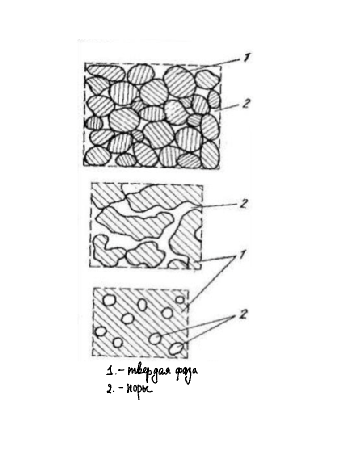
\includegraphics[width=0.2\textwidth]{chem_19_1.png}
    \end{center}
\end{wrapfigure}

\textbf{Ниже представлены основные стадии спекания.}



\textbf{Стадии спекания}


\begin{enumerate}
    \item стадия. \textbf{Припекание}. Создаются и увеличиваются контакты между соседними частицами, но границы зёрен сохраняются. \textit{Движущая сила спекания} --- избыток свободной энергии, связанной с дисперсностью порошка.
    \item стадия. \textbf{Обособление <<фазы вещества>> и <<фазы пустоты>>}. Частицы как бы сливаются, но замкнутых пор ещё не образуется. \textit{Движущая сила спекания} --- избыток энергии свободных поверхностей пор и межзёренных границ.
    \item стадия. Образуются замкнутые поры. \textit{Движущая сила спекания} --- уменьшение протяжённости границы раздела пор кристалла и удаление пор.
    \item студия. Удаления замкнутых пор.
\end{enumerate}


Явления, сопровождающие отжиг 1-го рода:

\begin{enumerate}
    \item Возврат (recovery) --- совокупность процессов самопроизвольного изменения плотности и распределения дефектов (и соответствующих им полей напряжений) в неравновесных (в частности, деформированных) кристаллах до начала рекристаллизации
    \begin{enumerate}
        \item возврат 1-го рода (отдых) --- без миграции малоугловых границ (дислокаций)
        \item возврат 2-го рода (полигонизация) --- миграция малоугловых границ (дислокаций)
    \end{enumerate}
    \item Рекристаллизация --- возникновение новых зерен, рост зерен (grain growth), сопровождающиеся движением высокоугловых границ
    \item Уплотнение (densification) --- уменьшение доли и размера пор
    \item Коалесценция пор (coarsening) --- укрупнение пор без изменения их общего объема
\end{enumerate}

\begin{figure}[h!]
    \centering
    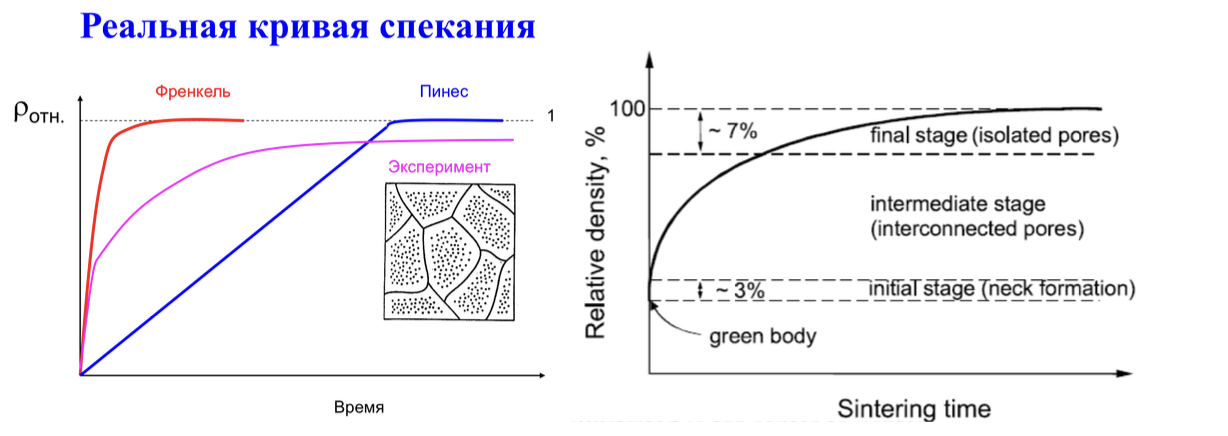
\includegraphics[width=0.8\textwidth]{chem_19_2.png}
\end{figure}


\section{Распад пересыщенного твердого раствора по спинодальному механизму и механизму образования и роста зародышей. Термодинамика процессов распада, роль упругой энергии. Старение материалов естественное и искусственное (на примере дуралюмина).}


\begin{wrapfigure}{r}{0.5\textwidth}
    \begin{center}
        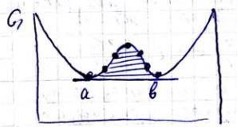
\includegraphics[width=0.4\textwidth]{chem_20_2.jpg}
    \end{center}
\end{wrapfigure}

Термодинамика: фазовая диаграмма и зависимость $G$ от состава. Если в пересыщенном растворе возникает флуктуация состава (в точке К), то в дальнейшем процесс будет происходить самопроизвольно (неустойчивое равновесие в очке К).

\begin{figure}[h!]
    \centering
    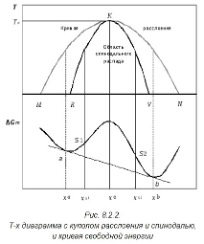
\includegraphics[width=0.4\textwidth]{chem_20_1.jpg}
\end{figure}


Флуктуация состава неравновесна, термодинамически выгоден распад: будет спонтанный постепенный распад на а и b --- \textbf{спинодальный распад} (граница растворимости в твердом состоянии):





\begin{wrapfigure}{r}{0.5\textwidth}
    \begin{center}
        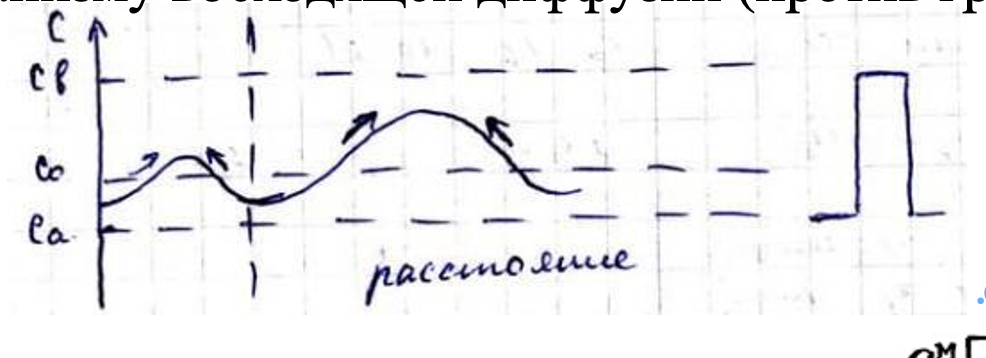
\includegraphics[width=0.4\textwidth]{chem_20_3}
    \end{center}
\end{wrapfigure}

Процесс протекает по механизму восходящей диффузии (против градиента концентраций). Справа --- состав, каким он будет по прошествии бесконечно большого интервала времени.

\textbf{Образование и рост зародышей }

\begin{wrapfigure}{r}{0.4\textwidth}
    \begin{center}
        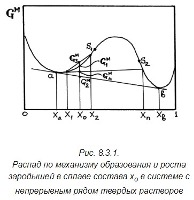
\includegraphics[width=0.4\textwidth]{chem_20_4}
    \end{center}
\end{wrapfigure}

Если происходит распад раствора, отвечающего точке $X_0$, то видно, что малые флуктуации состава термодинамически не выгодны, энергия системы кристаллов выше, чем у исходного раствора (ситуация 1). 

% \begin{wrapfigure}{r}{0.3\textwidth}
%     \begin{center}
%         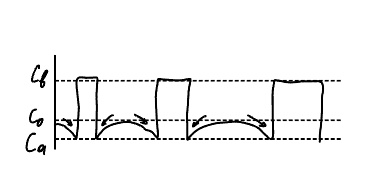
\includegraphics[width=0.4\textwidth]{chem_20_5}
%     \end{center}
% \end{wrapfigure}

\textbf{Для распада} (на $b$ и состав от $a$ до $X_0$) надо преодолеть некий энергетический барьер, необходимо присутствие зародышей новой фазы. Зародыши могут образовываться за счет сегрегации одного из компонентов на дислокациях, границах зерен и других дефектов. Этот процесс не захватывает весь объем, протекает по механизму нисходящей диффузии (по градиенту концентрации).


\pagebreak
\textbf{Сравнение двух процессов}

\begin{table}[h!]
    \centering
    \resizebox{\textwidth}{!}{
    \begin{tabular}{|c|c|}
    \hline
    Спинодальный распад & Образование и рост зародышей \\ \hline
    Флуктуации возникают где угодно & \makecell{Рост зародыша происходит в \\ выделенной зоне (поверхность границы зёрен)} \\ \hline \xrowht{15pt}

    $\frac{\partial ^2 C}{\partial C^2} = 0$ & $0=\frac{\partial G}{\partial C} \leftarrow C\frac{\partial ^2 C}{\partial C^2}$ \\ \hline

    \makecell{$D<0$, против градиента концентрации \\ восходящая дифузия} &  \makecell{$D>0$, по градиенту концентрации \\ нисходящая дифузия} \\ \hline

    Малые флуктуации состава & Зародыш новой фазы\\ \hline

    Состав фазы меняется & $C_a, C_b = const$ \\ \hline
    Размытая граница & Резкая граница \\ \hline

    \makecell{Когерентная граница \\ (сопряжение двух кристаллических решёток)} & $\pm$ \\ \hline

    $\pm$ & \makecell{Наступает термодинамическое \\ равновесие} \\ \hline

    \makecell{Закономерная пространственная \\ ориентация фаз} & $\pm$ \\ \hline
    
\end{tabular}}
\end{table}

\textbf{Термодинамика процессов распада, роль упругой энергии}

\begin{wrapfigure}{r}{0.5\textwidth}
    \begin{center}
        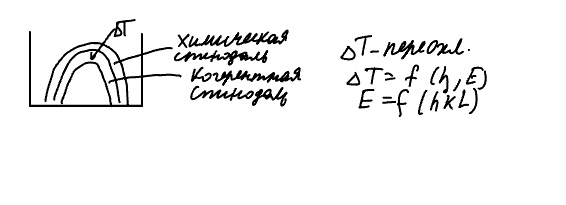
\includegraphics[width=0.5\textwidth]{chem_20_6}
    \end{center}
\end{wrapfigure}

Энергетика процесса спинодального распада определяется вкладом 3х компонент: объемной, поверхностной и упругой: $G= G^\text{об} + G^\text{пов} + G^\text{упр}$. Чем больше удельное изменение параметров решетки, с изменением состава  = $1/a \cdot da dc $ и чем жестче решетка (жесткость решётки определяется E --- модулем Юнга(!)) , тем больше вклад $ G^\text{упр}$. Энергия, выделяющаяся при распаде тратится на деформацию, поскольку изменяются параметры кристаллической решетки. Поэтому в реальности вместо химической спинодали наблюдается когерентная, которая лежит ниже по температуре. 

\textbf{Старение материалов: }
\begin{itemize}
    \item Естественное остаривание: при комнатной температуре, рост выделений внутри зерен.
    \item Искусственное остаривание: при комнатной температуре, рост выделений по границам зерен.  
\end{itemize}


\textbf{На примере дюралюминия (Сплав Cu-Al)}

Только что приготовленный дюралюмин мягкий. При выдерживании его в течение некоторого времени (остаривании) происходит распад твёрдого раствора (спинодальный), при этом возникают мелкие области (20-50~\si{\angstrom} неоднородности), обогащенные медью --- зоны Гинье-Престона (зоны Гинье-Престона --- см. следующий билет) (медь собирается в кластеры --- дискообразные частицы). Медь локализуется в дискообразных кластерах, решетка деформируется. Попадание внутрь купола (см. ниже) --- появление зон Гинье-Престона. Состав неравновесных кластеров может сильно различаться. При остаривании материал упрочняется. Сплав Cu-Al обладает повышенной твердостью и тягучестью (после остаривания).

\textbf{Реальная морфология:}

\begin{figure}[h!]
    \centering
    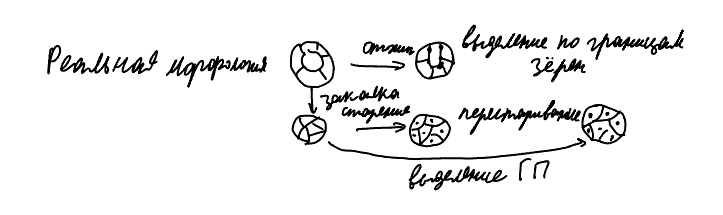
\includegraphics[width=0.9\textwidth]{chem_20_7}
\end{figure}


\section{Зональная стадия распада твердого раствора; термодинамика и кинетика образования и строение зон Гинье-Престона. Природа упрочнения при дисперсионном старении.}

\textbf{Остаривание} --- (в билете 20) выдерживание материала при невысокой температурах длительное время.

2 основных механизма: 

\begin{enumerate}
    \item \textbf{химический:} при пластической деформации некоторые дислокации проходят через область  зоны, 	поэтому 	будет 	осуществляться пластический сдвиг (дислокация <<перерезает>> зону)
   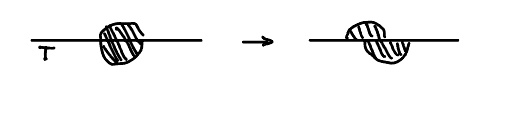
\includegraphics[width=0.5\textwidth]{chem_21_1}

    \item \textbf{механизм Орована:} образуется скопление частиц --- дислокация подходит к частицам и <<выгибается>>.
    
    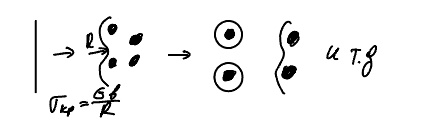
\includegraphics[width=0.3\textwidth]{chem_21_2}
\end{enumerate}




При высоких температурах зависимость проходит через максимум. Увеличивается количество частиц, они разрастаются и коалисцируют.

\begin{figure}[h!]
    \centering
    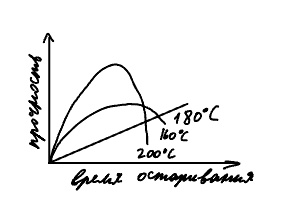
\includegraphics{chem_21_3}
\end{figure}



При высоких температурах механизм Орована вносит незначительный вклад, так как при коалисцировании уменьшается общее число частиц. 


\begin{wrapfigure}{r}{0.4\textwidth}
    \begin{center}
        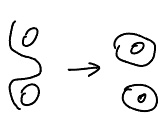
\includegraphics{chem_21_4}
    \end{center}
\end{wrapfigure}

\textbf{Упрочнение:}
\begin{enumerate}
    \item Выделяющаяся частица имеет больший модуль сдвига, что останавливает дислокации.
    \item Количество выделений (механизм Орована). Дислокации могут остановиться и могут пройти (схема на рисунке).
    \item Зависимость от температуры: сначала прочность растет (выделение мелких частиц), затем снижается (рост включений).
\end{enumerate}

\begin{figure}[h!]
    \centering
    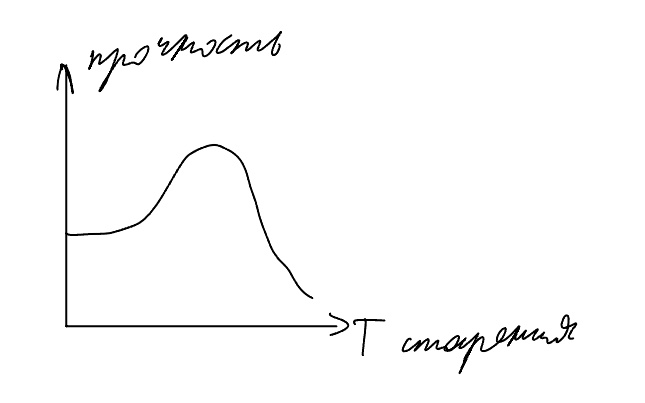
\includegraphics[width=0.6\textwidth]{chem_21_5}
\end{figure}



\section{Принципы химико--термической обработки. Виды термомеханической обработки материалов.}

\textbf{Типичные виды химико--термической обработки}

\begin{enumerate}
    \item цементация (закалка) (насыщение стали углеродом на поверхности). Закалка осуществляется в разной степени в зависимости от содержания углерода.
    \item азотирование (насыщение стали азотом).
    \item цеонирование 	(азотирование и цементация).
    
\end{enumerate}

\textbf{Механизм ХТО}

\begin{enumerate}
    \item выдерживание стальной болванки в соответствующей атмосфере.
    \item Происходит насыщение металла углеродом и (или) азотом --- 
диффузионный процесс.
    \item В результате получаем градиентный материал (состав разный на разном расстоянии от поверхности).  
\end{enumerate}

\textbf{Виды термомеханической обработки (ТМО) материалов}

\begin{enumerate}
    \item ВТМО --- высокотемпературная ($T>T_\text{эвтект}$) --- непосредственно после горячего воздействия давлением (пока аустенитная структура), проводится закалка. Не успевает произойти рекристаллизация.
    \begin{itemize}
        \item \textit{Наклёп} --- упрочнение металлов и сплавов в процессе пластической деформации при температуре ниже температуры рекристаллизации.
        \item \textit{Штамповкой} --- способ изготовления деталей давлением при металлических форм, очертания которых соответствуют очертаниям изготовляемых деталей. 
        \item \textit{Прокаткой} --- обработка давлением путем пропускания его в горячем или в холодном состоянии между вращающимися валками прокатного станка. 
        \item \textit{Рекристаллизация} --- процесс образования и роста (или только роста) одних кристаллических зёрен (кристаллитов) поликристалла за счёт других.
    \end{itemize}
    Наклеп и упрочнение не устраняются и остаются в материале после его остывания.  Чем короче промежуток времени между окончанием всех процессов, когда сталь имеет высокую температуру, тем больше сохранится дислокаций и тем больше будет эффект упрочнения.

    \begin{figure}[h!]
        \centering
        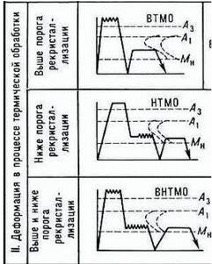
\includegraphics{chem_21_6}
    \end{figure}

    \item НТМО --- низкотемпературная ($T<T_\text{эвтект}$) 
    При низкотемпературной термомеханической обработке металл нагревают до аустенитного состояния, затем охлаждают ниже температуры рекристаллизации, но выше температуры начала мартенситного превращения, то есть температурный интервал пластической деформации составляет примерно 400--600~$\rm ^\circ C$. 
    
\end{enumerate}




Деформация, как и при ВТМО, вызывает наклеп аустенита, рекристаллизации же в этих условиях не происходит. Затем проводится закалка: образуется мартенсит, который, как и в предыдущем способе, наследует дислокации, а значит и упрочнение, полученное при низкотемпературной термомеханической обработке стали. Здесь устранен недостаток первого способа, так как рекристаллизация практически отсутствует и потому наиболее полно используется эффект упрочнения от наклепа.

ТМО позволяет получить достаточно высокую прочность ($\sigma _\text{в}= 2200-3000$~МПа) при хорошей пластичности и вязкости ($\delta= 6 -8\%, \psi = 50-60\%)$. 
